\documentclass[mathserif]{beamer} 
\usepackage{eulervm} %красивый математический шрифт - по желанию
\usepackage{ulem} %зачёркивания
\usepackage{bm} %особо жирный математический
\usepackage{schemata} %для красивых блочных переходов, пользуюсь редко
\usepackage{mathtools} %улучшенная работа с типографией в math mode
\setbeamertemplate{navigation symbols}{} %отключает управляющие символы в правом нижнем углу
\usefonttheme{professionalfonts}
\usepackage{cmap} %чтобы были работающие гиперссылки
\usepackage{makeidx,fancybox,tikz}
\usetikzlibrary{automata, positioning, arrows,patterns}
\usetikzlibrary{arrows.meta}
\usepackage{tempora} %по желанию -- русские штрифты с засечками

\mode<presentation>
{
% \usetheme{Warsaw}
%  \usetheme{Frankfurt}
%  \usetheme{Singapore}
%  \usetheme{Boadilla}
%  \usetheme{Montpellier}
%  \usetheme{Szeged}
  \usetheme{CambridgeUS} %тут решайте сами, что выбрать
    % or ...

%  \usecolortheme{dolphin}
  \usecolortheme{dove} %аналогично
%  \usecolortheme{wolverine}
%  \usecolortheme{crane}

%  \usefonttheme{structurebold}
%  \usefonttheme{structuresmallcapsserif}

%  \setbeamercovered{transparent}
}
\usepackage[T1,T2A]{fontenc}
\usepackage[utf8]{inputenc}
\usepackage[english,russian]{babel}
\usepackage{amsmath,mathrsfs} %ещё больше математических символов
\usepackage{amstext}
\usepackage{graphicx,relsize}
\graphicspath{ {./documentation/} }

\usepackage{color}
\definecolor{gray}{rgb}{0.4,.4,0.4} %здесь можно определить собственные цвета
\definecolor{grey80}{rgb}{0.8,.8,0.8}
\definecolor{grey90}{rgb}{0.9,.9,0.9}
\definecolor{grey95}{rgb}{0.95,.95,0.95}
\newcommand\redstroke{\bgroup\markoverwith
{\textcolor{red}{\rule[0.5ex]{2pt}{1.5pt}}}\ULon} %зачёркивание жирной красной чертой

\newcommand\reduline{\bgroup\markoverwith
{\textcolor{red}{\rule[-0.5ex]{2pt}{1.5pt}}}\ULon}%подчёркивание жирной красной чертой

\newcommand\bluline{\bgroup\markoverwith
{\textcolor{blue}{\rule[-0.5ex]{2pt}{1.5pt}}}\ULon}

\newcommand\bolduline{\bgroup\markoverwith
{\textcolor{white}{\rule[-0.5ex]{2pt}{1.5pt}}}\ULon}

\title[] {Follow-автомат (IlieYu)}

\author[Chipollino]{Лучшая команда разработчиков по ТФЯ} % :))
\date[] 
{2022 г.}
\subject{Computer Science}

\newcommand{\Lang}{\mathscr{L}} %макрос для языка регулярки или автомата
\def\logor{\mathrel{\vee}} %отрендеренные логические операторы (с правильными интервалами)
\def\logimpl{\mathrel{\Rightarrow}}
\def\Linearize{\mathtt{Linearize}} %названия операций интерпретатора записываем моноширинным
\def\First{\mathrm{First}} %названия прочих операций записываем обычным шрифтом, но не тем, который в math mode по умолчанию
\def\Last{\mathrm{Last}}
\def\Follow{\mathrm{Follow}}
\def\IlieYu{\mathrm{IlieYu}}
\def\Glushkov{\mathtt{Glushkov}}
\def\Thompson{\mathtt{Thompson}}
\def\logand{\mathrel{\&}}
\def\lognot{\mathop{\neg}}
\def\iff{\mathrel{\Leftrightarrow}}
\def\quantall#1{\mathop{\forall #1}}
\def\quantex#1{\mathop{\exists #1}} 
\def\alter{\ensuremath{\mathrel{\vert}}}%отрендеренные регулярные операторы 
\def\star{\ensuremath{^{*}}}%отрендеренные регулярные операторы 
\def\regexpstr#1{\mathtt{#1}}%буквы внутри регулярок переписываются в моноширинный
\newcommand{\Nat}{\mathbb N}
\newcommand{\empt}{\varepsilon} %пустое слово
\newcommand{\bottom}{\bot} %противоречие
\newcommand{\rar}{\rightarrow} %стрелка вправо. Для экономии букв.
\newcommand{\RegExp}{\mathcal{RE}} %макрос для обозначения множества всех регулярок
%в преамбулу можно и нужно добавлять свои макросы

\begin{document}

\maketitle
\section{Основные понятия}
\begin{frame}{Follow-эквивалентность}
    \begin{block}{\bf Определение}
        Пусть $R$ --- регулярное выражение. Положим $follow(a_{i}) = \{a_{j} | \exists w, u(wa_{i}a_{j}u \in\Lang(R))\}$.

        Follow-эквивалентность: состояния автомата Глушкова $a_{i}$ и $a_{j}$ follow-эквивалентны, если $follow(a_{i}) = follow(a_{j})$, и либо $a_{i}$, $a_{j}$ оба финальные, либо они оба не финальные.
    \end{block} % descriptive documentation
\end{frame}

\section{Follow-автомат (IlieYu)}
\begin{frame}{Конструкция автомата Илия-Ю (или follow-автомата)}
    \begin{block}{\bf Алгоритм построения $\IlieYu(r)$}
        \begin{itemize}
            \item Построить автомат Глушкова ($\Glushkov$);
            \item Объединить follow-эквивалентные состояния.
        \end{itemize}
    \end{block} % descriptive documentation
\end{frame}

%Здесь я включила граф, порождённый скриптом dot2tex, и разница с простым Graphviz-овским по оформлению меток и т.п. очень заметна. Но dot2tex, к сожалению, периодически лагает (хотя часть его багов, например, с конвертацией string->float, возникающей на метках, состоящих из нескольких цифр, исправляется переходом к чуть-чуть другому представлению в dot-файле). Зато красивый вектор и выравнивание.
%Можно сделать html-метки в графвизовском представлении (это позволит делать нижние индексы, например) и вставлять картинки. Вид будет немного не такой "стильный", но приемлемый. 
%Можно совместить оба подхода: если получается породить tikz-исходник, то переносить его в tex-исходник документа, в противном случае вставлять Graphviz. Для единообразия, чтобы не было смеси того и другого, можно вставлять Graphviz везде, если dot2tex зафейлился хотя бы на одном графе.
\begin{frame}{Пример Follow-автомата (IlieYu)}
    % \vspace{-5pt}
    Исходное регулярное выражение:

    \[(\regexpstr{a}\alter \regexpstr{b})\star\regexpstr{b}\]% the initial regexp placeholder displaystyle

    Автомат Глушкова:

    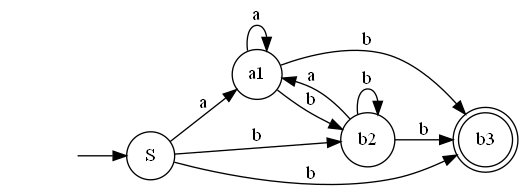
\includegraphics[width=2in, keepaspectratio]{follow1.png}

    Follow-отношения:
    \begin{itemize}
        \item $S$: $a_{1}$ $b_{2}$ ;
        \item $b_{3}$: ;
    \end{itemize}

\end{frame}%overall documentation

\begin{frame}{Пример автомата Follow-автомат (IlieYu)}
    Follow-автомат:

    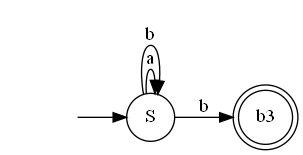
\includegraphics[width=2in, keepaspectratio]{follow2.png}

\end{frame}%overall documentation

% overall documentation : section 
\section{Обсуждение}
%В разделе "обсуждение" можно добавлять всё что угодно по вкусу: историческую справку, какие-то интересные примеры, способы применения, связь с другими понятиями теории автоматов и т.д. Можно сделать дополнительный метакомментарий: basic documentation, добавляющую ещё какие-то простые пояснения.
\begin{frame}{Cвойства Follow-автомат (IlieYu)}
    \begin{itemize}
        \item Если написал автомат Глушкова, то писать Follow-автомат просто сказка (по словам господина Князихина)
        \item а его свойств я не знаю
    \end{itemize}
\end{frame}
\end{document}
